\documentclass[tikz,border=10pt]{standalone}
\usepackage{tikz,amsmath}
\usetikzlibrary{arrows.meta,positioning,calc,fit}
\begin{document}
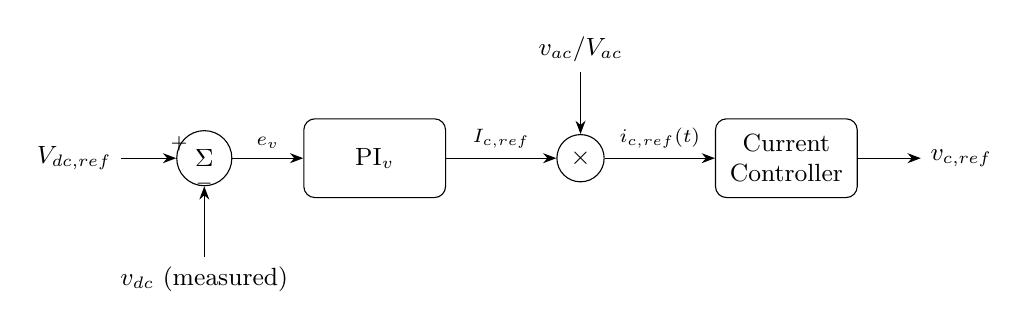
\begin{tikzpicture}[
  font=\small,
  >=Stealth,
  block/.style={draw, rounded corners, minimum width=1.8cm, minimum height=1.0cm, align=center},
  sum/.style={draw, circle, inner sep=0pt, minimum size=0.7cm},
  mul/.style={draw, circle, inner sep=0pt, minimum size=0.6cm},
  dot/.style={circle, fill=black, inner sep=0pt, minimum size=3pt},
]

% Row: V_dc,ref -> sum -> PI_v -> (I_c,ref) -> x (v_ac/V_ac) -> i_c,ref(t) -> Current Controller -> v_c,ref
\node                      (Vref) at (0, 0)   {$V_{dc,ref}$};
\node[sum, right=0.7cm of Vref]  (S1)         {$\Sigma$};
\node[block, right=0.9cm of S1]  (PI)         {$\mathrm{PI}_v$};
\node[mul, right=1.4cm of PI]    (M1)         {$\times$};
\node[block, right=1.4cm of M1]  (CC)         {Current\\Controller};

% Sum signs
\node[font=\scriptsize] at ($(S1) + (-0.32, 0.18)$) {$+$};
\node[font=\scriptsize] at ($(S1) + (0, -0.32)$)    {$-$};

% Feedback into sum
\node[below=0.9cm of S1] (vdc_meas) {$v_{dc}$ (measured)};
\draw[->] (vdc_meas) -- (S1);

% Input to multiplier from above: v_ac/V_ac
\coordinate (mul_in) at ($(M1) + (0, 1.1)$);
\node[above] at (mul_in) {$v_{ac}/V_{ac}$};
\draw[->] (mul_in) -- (M1);

% Wires left-to-right
\draw[->] (Vref) -- (S1);
\draw[->] (S1)   -- node[above, font=\scriptsize]{$e_v$} (PI);
\draw[->] (PI)   -- node[above, font=\scriptsize]{$I_{c,ref}$} (M1);
\draw[->] (M1)   -- node[above, font=\scriptsize]{$i_{c,ref}(t)$} (CC);

% Output from Current Controller
\node[right=0.8cm of CC] (vcref) {$v_{c,ref}$};
\draw[->] (CC) -- (vcref);

\end{tikzpicture}
\end{document}
